% docs/slides/preamble.tex -- 五份 deck 共享
\documentclass[aspectratio=169,11pt]{beamer}

% ==== 中文与字体 ====
\usepackage[UTF8,fontset=none]{ctex}
\usepackage{fontspec}

\IfFontExistsTF{PingFang SC}{%
  \setCJKmainfont{PingFang SC}[BoldFont=PingFang SC,ItalicFont=PingFang SC,AutoFakeSlant=0.15]
  \setCJKsansfont{PingFang SC}[ItalicFont=PingFang SC,AutoFakeSlant=0.15]
  \setCJKmonofont{PingFang SC}
}{%
  \IfFontExistsTF{Source Han Sans SC}{%
    \setCJKmainfont{Source Han Sans SC}
    \setCJKsansfont{Source Han Sans SC}
  }{%
    \IfFontExistsTF{Noto Sans CJK SC}{%
      \setCJKmainfont{Noto Sans CJK SC}
      \setCJKsansfont{Noto Sans CJK SC}
    }{%
      \setCJKmainfont{Heiti SC}
      \setCJKsansfont{Heiti SC}
    }
  }
}

\IfFontExistsTF{Helvetica Neue}{\setmainfont{Helvetica Neue}}{%
  \IfFontExistsTF{Inter}{\setmainfont{Inter}}{}}
\IfFontExistsTF{JetBrains Mono}{\setmonofont{JetBrains Mono}[Scale=0.85]}%
  {\setmonofont{Menlo}[Scale=0.85]}

% ==== 颜色 ====
\usepackage{xcolor}
\definecolor{cMain}{HTML}{1F4E79}
\definecolor{cAccent}{HTML}{E07A1F}
\definecolor{cGray}{HTML}{595959}
\definecolor{cMute}{HTML}{F4F4F4}
\definecolor{cOK}{HTML}{2E7D32}
\definecolor{cBad}{HTML}{B23A3A}
\definecolor{cWarn}{HTML}{C8A300}

% ==== 主题 ====
\usepackage{tcolorbox}
\usetheme{metropolis}
\metroset{progressbar=frametitle,numbering=fraction,block=fill}
\setbeamercolor{frametitle}{bg=cMain,fg=white}
\setbeamercolor{progress bar}{fg=cAccent,bg=cMute}
\setbeamercolor{alerted text}{fg=cAccent}
\setbeamercolor{title}{fg=cMain}

% metropolis 默认尝试 Fira Sans，未安装时 fallback 到 Latin Modern Sans。
% 这里在主题加载后显式覆盖，强制使用 macOS 上一定存在的 Helvetica Neue，
% 跟中文 PingFang 风格一致；找不到则按顺序尝试 Inter / Arial。
\IfFontExistsTF{Helvetica Neue}{%
  \setsansfont{Helvetica Neue}%
}{%
  \IfFontExistsTF{Inter}{\setsansfont{Inter}}{%
    \IfFontExistsTF{Arial}{\setsansfont{Arial}}{}}%
}

% ==== TikZ ====
\usepackage{tikz}
\usetikzlibrary{positioning,arrows.meta,fit,shapes.geometric,calc,%
  decorations.pathmorphing,backgrounds}

\tikzset{
  node-box/.style={draw=cMain,thick,rounded corners=2pt,
    minimum height=8mm,minimum width=18mm,align=center,font=\small},
  node-state/.style={draw=cMain,thick,circle,minimum size=14mm,
    align=center,font=\small},
  node-ok/.style={draw=cOK,thick,fill=cOK!10},
  node-warn/.style={draw=cWarn,thick,fill=cWarn!15},
  node-bad/.style={draw=cBad,thick,fill=cBad!10},
  % 色盲友好的状态机三态：蓝 (正常/Closed) / 橙 (告警/Open) / 灰 (中间/HalfOpen)
  % 避免 red-green 二元区分，改用 hue + lightness 双通道。
  node-state-normal/.style={draw=cMain,thick,fill=cMain!12},
  node-state-alert/.style={draw=cAccent,thick,fill=cAccent!18},
  node-state-transition/.style={draw=cGray,thick,fill=cGray!18},
  arrow/.style={-{Stealth[length=2mm]},thick,draw=cMain},
  arrow-async/.style={-{Stealth[length=2mm]},thick,dashed,draw=cGray},
  arrow-bad/.style={-{Stealth[length=2mm]},thick,draw=cBad},
  arrow-alert/.style={-{Stealth[length=2mm]},thick,draw=cAccent},
  lifeline/.style={dashed,thick,draw=cGray},
}

% ==== 代码 ====
\usepackage{listings}
\lstdefinelanguage{Go}{
  morekeywords={break,case,chan,const,continue,default,defer,else,
    fallthrough,for,func,go,goto,if,import,interface,map,package,range,
    return,select,struct,switch,type,var,nil,true,false,iota},
  morekeywords=[2]{string,int,int64,uint,uint64,bool,byte,error,context},
  sensitive=true,
  morecomment=[l]//,morecomment=[s]{/*}{*/},
  morestring=[b]",morestring=[b]`,
}
\lstdefinelanguage{LuaRedis}{
  morekeywords={and,break,do,else,elseif,end,false,for,function,if,in,
    local,nil,not,or,repeat,return,then,true,until,while},
  morekeywords=[2]{redis,call,KEYS,ARGV,tonumber,HGET,HSET,GET,SET,
    DECR,DECRBY,INCR,INCRBY,EXPIRE,PEXPIRE,ZADD,ZCARD,ZREMRANGEBYSCORE,
    EVAL,EVALSHA},
  sensitive=true,
  morecomment=[l]{--},
  morestring=[b]",morestring=[b]',
}

\lstdefinestyle{base}{
  basicstyle=\ttfamily\scriptsize,
  numbers=left,numberstyle=\tiny\color{cGray},
  keywordstyle=\color{cMain}\bfseries,
  keywordstyle=[2]\color{cAccent},
  stringstyle=\color{cOK},
  commentstyle=\color{cGray}\itshape,
  backgroundcolor=\color{cMute},
  frame=single,framerule=0pt,
  showstringspaces=false,
  breaklines=true,
  tabsize=2,
  columns=fullflexible,
}
\lstset{style=base}

% ==== 三线表与附录页码 ====
\usepackage{booktabs}
\usepackage{appendixnumberbeamer}

% ==== 页脚来源标注 ====
\newcommand{\srcnote}[1]{{\color{cGray}\scriptsize\itshape #1}}

% 关键论点框
\newcommand{\keypoint}[1]{%
  \begin{tcolorbox}[colback=cMute,colframe=cMain,boxrule=0.5pt,arc=2pt]%
  #1\end{tcolorbox}}


\title{付完款只是开始}
\subtitle{电商履约链路全景与 gomall 路线图 (业务侧 deck)}
\author{gomall · 业务侧 deck}
\date{}

\begin{document}

\maketitle

\begin{frame}{今日大纲}
\tableofcontents
\end{frame}

% ============================================================
\section{业务困局与完整状态机}
% ============================================================

\begin{frame}{客服后台每天收到的三类工单}
\begin{tikzpicture}[node distance=4mm and 6mm,every node/.style={font=\scriptsize}]
  \node[node-box,minimum width=38mm,node-bad] (c1) {"付完款 App 还显示订单待支付"};
  \node[node-box,minimum width=38mm,node-bad,right=of c1] (c2) {"已付款 5 天没发货"};
  \node[node-box,minimum width=38mm,node-bad,right=of c2] (c3) {"签收时东西已经坏了"};
  \node[node-box,minimum width=120mm,below=8mm of c2,node-warn] (root)
    {根因：履约链路缺位——订单状态机停在"付款"那一步，没有继续走};
  \draw[arrow-bad] (c1) -- (root.north -| c1);
  \draw[arrow-bad] (c2) -- (root.north -| c2);
  \draw[arrow-bad] (c3) -- (root.north -| c3);
\end{tikzpicture}
\vspace{2mm}
\begin{itemize}
  \item C1 是支付到订单同步\textbf{慢/丢}：典型对账问题，已付款事件没及时落到订单上。
  \item C2 是发货 SLA 缺失：商家什么时候必须发货，平台没承诺、没监控。
  \item C3 是签收和售后链路缺失：东西坏了走哪条退货流程，没定义。
\end{itemize}
\srcnote{consts/order.go:11--15 当前状态枚举只有 UnPaid / Paid / Cancelled / Refunded}
\end{frame}

\begin{frame}{电商订单状态机：完整版}
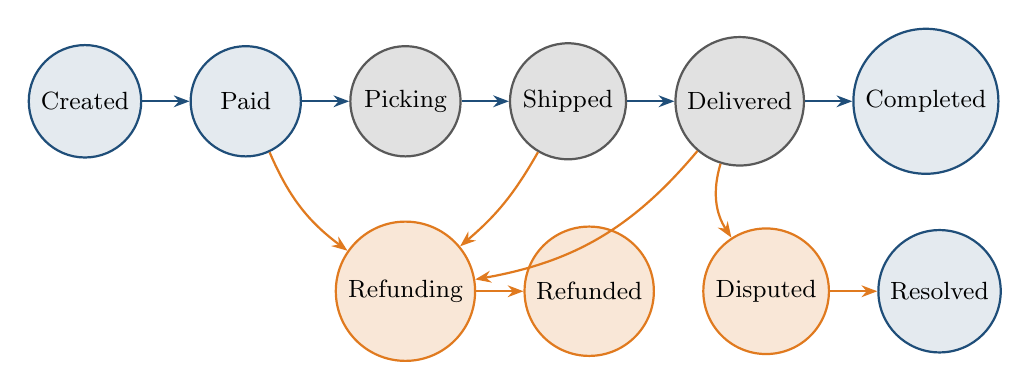
\begin{tikzpicture}[node distance=4mm and 6mm,every node/.style={font=\scriptsize}]
  \node[node-state,node-state-normal] (cr)  {Created};
  \node[node-state,node-state-normal,right=of cr]   (pd)  {Paid};
  \node[node-state,node-state-transition,right=of pd]   (pk)  {Picking};
  \node[node-state,node-state-transition,right=of pk]   (sh)  {Shipped};
  \node[node-state,node-state-transition,right=of sh]   (dv)  {Delivered};
  \node[node-state,node-state-normal,right=of dv]   (cp)  {Completed};
  \node[node-state,node-state-alert,below=8mm of pk]   (rf)  {Refunding};
  \node[node-state,node-state-alert,right=of rf]   (rd)  {Refunded};
  \node[node-state,node-state-alert,right=of rd]   (dp)  {Disputed};
  \node[node-state,node-state-normal,right=of dp]  (rs)  {Resolved};
  \draw[arrow] (cr) -- (pd);
  \draw[arrow] (pd) -- (pk);
  \draw[arrow] (pk) -- (sh);
  \draw[arrow] (sh) -- (dv);
  \draw[arrow] (dv) -- (cp);
  \draw[arrow-alert] (pd) to[bend right=15] (rf);
  \draw[arrow-alert] (sh) to[bend left=10]  (rf);
  \draw[arrow-alert] (dv) to[bend left=20]  (rf);
  \draw[arrow-alert] (rf) -- (rd);
  \draw[arrow-alert] (dv) to[bend right=25] (dp);
  \draw[arrow-alert] (dp) -- (rs);
\end{tikzpicture}
\vspace{1mm}
\small 主链 6 态 \texttt{Created $\to$ Paid $\to$ Picking $\to$ Shipped $\to$ Delivered $\to$ Completed}；
分支两条：\texttt{Refunding $\to$ Refunded}（金额回退）和 \texttt{Disputed $\to$ Resolved}（售后争议）。
\srcnote{京东/淘宝/天猫公开订单 API 状态枚举 综合归纳}
\end{frame}

\begin{frame}{gomall 现状与差距对照}
\begin{tikzpicture}[node distance=3mm and 10mm,every node/.style={font=\tiny}]
  \node[node-state,node-state-normal,minimum size=11mm] (u) {UnPaid};
  \node[node-state,node-state-normal,minimum size=11mm,right=of u] (p) {Paid};
  \node[node-state,node-state-transition,minimum size=11mm,right=of p] (c) {Cancelled};
  \node[node-state,node-state-alert,minimum size=11mm,right=of c] (r) {Refunded\\\tiny 占位};
  \draw[arrow] (u) -- (p);
  \draw[arrow-alert] (u) to[bend right=20] (c);
  \draw[arrow,dashed] (p) -- (r);
\end{tikzpicture}
\vspace{1mm}
{\scriptsize
\begin{tabular}{@{}llll@{}}
\toprule
完整链路 & gomall & 缺失原因 & 客诉表现 \\
\midrule
Created/Paid       & \checkmark                  & ---            & --- \\
Picking            & \textbf{缺}                 & 仓储未接        & "下单后没动静" \\
Shipped            & \textbf{缺}                 & 物流单未建      & "5 天没发货" \\
Delivered          & \textbf{缺}                 & 物流回调未接    & "看不到包裹到哪" \\
Completed          & \textbf{缺}                 & 收货确认未做    & "钱啥时放给商家" \\
Refunding/Refunded & 枚举有 / 无写入             & 退款 Saga 未做  & "退款卡住" \\
\bottomrule
\end{tabular}
}
\vspace{1mm}
\small 缺 \textbf{4--5 个核心状态}。每一个缺位对应至少一类客诉。
\srcnote{consts/order.go:4--7, 11--15}
\end{frame}

% ============================================================
\section{履约五段拆解与现有积木}
% ============================================================

\begin{frame}{把"付款到收货"切成五段}
\begin{tabular}{@{}lp{4.2cm}p{4.4cm}@{}}
\toprule
阶段 & 业务动作 & gomall 现状 \\
\midrule
仓储   & 库存预扣 $\to$ 实扣 $\to$ 拣货单            & 预扣有，拣货单 \textbf{缺} \\
出库   & 拣货 $\to$ 复核 $\to$ 打包 $\to$ 出库单     & \textbf{全缺} \\
物流   & 物流单 $\to$ 揽收 $\to$ 中转 $\to$ 派送     & \textbf{全缺} \\
签收   & 收件人确认 $\to$ 订单推进 Completed         & \textbf{缺} \\
售后   & 退换货 $\to$ 退款 Saga                       & \textbf{缺} \\
\bottomrule
\end{tabular}
\vspace{1mm}
\small "缺"的根因不是技术做不到 —— MVP 阶段先聚焦\textbf{交易闭环}，履约依赖第三方仓 / 物流。自营 SKU 占比上来后五段都要补。
\srcnote{repository/cache/inventory.go:11--14 库存双桶模型 (available/reserved)}
\end{frame}

\begin{frame}{阶段 1 仓储：唯一已经站住的一段}
\begin{tikzpicture}[node distance=6mm and 10mm]
  \node[node-box] (cr) {下单};
  \node[node-box,right=of cr,node-warn] (av) {available};
  \node[node-box,right=of av,node-warn] (rv) {reserved};
  \node[node-box,right=of rv,node-ok]   (pd) {已支付\\\scriptsize commit};
  \node[node-box,below=of rv,node-bad]  (cc) {未付取消\\\scriptsize release};
  \draw[arrow] (cr) -- (av);
  \draw[arrow] (av) -- node[above,font=\tiny]{Reserve} (rv);
  \draw[arrow] (rv) -- node[above,font=\tiny]{Commit} (pd);
  \draw[arrow-bad] (rv) -- node[right,font=\tiny]{Release} (cc);
\end{tikzpicture}
\vspace{1mm}
\begin{itemize}
  \item Redis 双桶模型 (\texttt{available} / \texttt{reserved}) 在下单 / 支付 / 关单三条路径上落实原子语义。
  \item \textbf{缺的不是"扣库存"，是"出库的下一步动作"}：拣货单（从哪个货架挑哪几件）。
  \item 自营仓场景下，拣货单是 WMS 的事；gomall MVP 没接 WMS，所以这一步只是\textbf{数字游戏}—— DB 里 \texttt{product.Num} 扣了，没有"物理上挑出来"这一步。
\end{itemize}
\srcnote{repository/cache/inventory.go:32--66 Reserve/Commit/Release Lua；service/payment.go:128--143 DB 真扣}
\end{frame}

\begin{frame}{阶段 2--5 的客诉成本}
\begin{tabular}{@{}llp{5.2cm}@{}}
\toprule
缺位环节 & 客诉成本 & 为什么 gomall 暂缺 \\
\midrule
出库单        & "已付款 5 天没发货"     & 平台未承诺出库 SLA，商家拖单无监控 \\
拣货 / 复核   & 错发 / 漏发 / 多发      & 自营仓未建，依赖商家自管 \\
物流建单      & "我的订单怎么没单号"    & 物流商接口未对接 \\
揽收 / 中转   & "包裹卡在路上没动"      & 物流商 webhook 未接 \\
签收确认      & "钱啥时放给商家"        & 无确认收货链路 \\
售后退换货    & "退款卡住" / "差评"     & Refunded 枚举无写入路径 \\
\bottomrule
\end{tabular}
\vspace{1mm}
\small 共性：\textbf{都依赖第三方 webhook 或客服后台}。一旦接入，回调可靠性、签名、重放、乱序就是新的工程难题。
\srcnote{routes/router.go 无 /logistics/* 路由；service/payment.go:104--126 付款即放款}
\end{frame}

\begin{frame}{gomall 已有积木一览}
\begin{tabular}{@{}lll@{}}
\toprule
积木 & 来自 & 履约场景里能干什么 \\
\midrule
Outbox 模式       & deck 04 / service/outbox & 跨服务事件投递 at-least-once \\
Saga 协同         & deck 04 / 事件驱动        & 退款 / 出库失败的多步回滚 \\
RMQ 延迟队列      & deck 15 / order\_delay   & 超时未发货 / 超时未签收 自动推进 \\
Cron 兜底         & deck 15 / order\_task    & RMQ 挂时的最后一道闸 \\
幂等 SQL          & deck 15 / WHERE 状态     & 物流回调重放安全 \\
库存双桶          & deck 11 / cache/inventory& 退款时把库存还回 available \\
\bottomrule
\end{tabular}
\vspace{1mm}
\small 履约链路新增代码量大，但\textbf{底层一致性机制不用重新造}：每一段都能从这六块积木里挑两三块拼起来。
\srcnote{service/outbox/publisher.go:39--62 现有 Publisher；repository/rabbitmq/order\_delay.go:24--56 延迟拓扑}
\end{frame}

\begin{frame}{Outbox + Saga 在履约链路里怎么用}
\begin{tikzpicture}[node distance=3mm and 6mm,font=\scriptsize,
    every node/.append style={minimum width=14mm,minimum height=7mm}]
  \node[node-box]                 (paid)  {OrderPaid\\事件};
  \node[node-box,right=of paid,node-warn]   (pick)  {生成\\拣货单};
  \node[node-box,right=of pick,node-warn]   (ship)  {生成\\出库单};
  \node[node-box,right=of ship,node-warn]   (lgs)   {建物流\\单};
  \node[node-box,right=of lgs,node-ok]      (st)    {推进\\Shipped};
  \node[node-box,below=of pick,node-bad]    (rb1)   {撤销\\拣货};
  \node[node-box,below=of ship,node-bad]    (rb2)   {撤销\\出库};
  \node[node-box,below=of lgs,node-bad]     (rb3)   {取消\\物流};
  \draw[arrow] (paid) -- (pick);
  \draw[arrow] (pick) -- (ship);
  \draw[arrow] (ship) -- (lgs);
  \draw[arrow] (lgs)  -- (st);
  \draw[arrow-bad,dashed] (pick) -- (rb1);
  \draw[arrow-bad,dashed] (ship) -- (rb2);
  \draw[arrow-bad,dashed] (lgs)  -- (rb3);
\end{tikzpicture}
\vspace{2mm}
\begin{itemize}
  \item 每一步都写一条新 outbox 事件 (\texttt{order.picking} / \texttt{order.shipped} / ...)。
  \item 任一步失败 $\to$ 走对应\textbf{补偿事件}（reverse arrow），最终回到一个一致状态。
  \item 协同式 Saga 没有中心 coordinator，靠 RMQ topic 串起来 —— 与 deck 04 现状一致。
\end{itemize}
\srcnote{service/events/events.go:1--33 现有事件；docs/slides/04-outbox-saga.tex \S Saga}
\end{frame}

\begin{frame}{RMQ 延迟队列的多场景复用}
\begin{tabular}{@{}lll@{}}
\toprule
场景 & 延迟 & 触发动作 \\
\midrule
30 分钟未付款       & 30 min  & CancelUnpaidOrder（已落地，deck 15） \\
72 小时商家未发货   & 72 h    & 自动通知 + 客服介入工单 \\
15 天未签收         & 15 d    & 自动确认收货 + 放款给商家 \\
30 天未发起售后     & 30 d    & 关闭售后入口 \\
\bottomrule
\end{tabular}
\vspace{2mm}
\small RMQ TTL + 死信交换的拓扑是\textbf{可复用}的：每个延迟场景只需要新加一对 \texttt{*.delay.queue / *.dead.queue}，PublishDelayed 函数签名一模一样。
\srcnote{repository/rabbitmq/order\_delay.go:24--56 拓扑模式可复刻}
\end{frame}

% ============================================================
\section{物流单 + 退款 Saga 路线图}
% ============================================================

\begin{frame}{物流单的最小业务字段}
\begin{tabular}{@{}ll@{}}
\toprule
字段 & 业务含义 \\
\midrule
\texttt{logistics\_no}      & 物流商单号（顺丰 SF... / 京东 JD...） \\
\texttt{carrier}            & 承运方编码（SF / JD / YTO / ...） \\
\texttt{from\_zone}         & 发货仓 / 起站 \\
\texttt{to\_zone}           & 收货地址 / 终站 \\
\texttt{status}             & 揽收 / 中转 / 派送 / 签收 / 异常 \\
\texttt{events[]}           & 节点时间线（时间、地点、动作） \\
\texttt{sla\_promised\_at}  & 平台承诺送达时间 \\
\bottomrule
\end{tabular}
\vspace{2mm}
\small \textbf{events[]} 是 append-only 节点流（类似消息队列），status 是 events 末态的物化视图。这种"事件流 + 物化态"模型与 gomall 现有的 outbox 设计天然契合。
\srcnote{未来 repository/db/model/logistics.go 设计草案}
\end{frame}

\begin{frame}{物流商 webhook $\to$ outbox 链路}
\begin{tikzpicture}[node distance=6mm and 10mm]
  \node[node-box,node-bad] (cr) {webhook\\\scriptsize 第三方推送};
  \node[node-box,right=of cr,node-warn] (gw) {接收\\\scriptsize 签名校验};
  \node[node-box,right=of gw,node-ok]   (ob) {写 outbox\\\scriptsize logistics.event};
  \node[node-box,right=of ob,node-ok]   (db) {DB tx\\\scriptsize append events[]};
  \node[node-box,below=of ob,node-warn] (cs) {消费者\\\scriptsize 推进订单状态};
  \node[node-box,right=of cs,node-ok]   (usr){推送用户\\\scriptsize "包裹已派送"};
  \draw[arrow]      (cr) -- (gw);
  \draw[arrow]      (gw) -- (ob);
  \draw[arrow]      (ob) -- (db);
  \draw[arrow-async](ob) -- (cs);
  \draw[arrow]      (cs) -- (usr);
\end{tikzpicture}
\vspace{1mm}
\begin{itemize}
  \item webhook 不可靠（重试 / 乱序 / 丢失）—— 用 \texttt{(logistics\_no, event\_seq)} 作幂等键。
  \item 落 outbox 而不是直接改订单：万一订单服务挂了，事件不会丢。
  \item 消费者负责把\textbf{物流节点}翻译为\textbf{订单状态推进}（揽收 $\to$ Shipped、签收 $\to$ Delivered）。
\end{itemize}
\srcnote{service/outbox/publisher.go:65--86 现有 publisher 模式可复用}
\end{frame}

\begin{frame}{退款发起后必须做的四件事}
\begin{tikzpicture}[node distance=6mm and 8mm,font=\scriptsize,
    every node/.append style={minimum width=17mm,minimum height=9mm}]
  \node[node-box]                       (apl) {1. 申请\\客服审核};
  \node[node-box,right=of apl,node-warn] (pay) {2. 第三方\\退款 API};
  \node[node-box,right=of pay,node-warn] (inv) {3. 库存\\回退};
  \node[node-box,right=of inv,node-warn] (ob)  {4. outbox\\refunded};
  \node[node-box,right=of ob,node-ok]    (ok)  {状态\\Refunded};
  \node[node-box,below=of pay,node-bad]  (cmp1){补偿\\回滚审核};
  \node[node-box,below=of inv,node-bad]  (cmp2){补偿\\重调退款};
  \node[node-box,below=of ob,node-bad]   (cmp3){补偿\\库存调整};
  \draw[arrow]      (apl) -- (pay);
  \draw[arrow]      (pay) -- (inv);
  \draw[arrow]      (inv) -- (ob);
  \draw[arrow]      (ob)  -- (ok);
  \draw[arrow-bad,dashed] (pay) -- (cmp1);
  \draw[arrow-bad,dashed] (inv) -- (cmp2);
  \draw[arrow-bad,dashed] (ob)  -- (cmp3);
\end{tikzpicture}
\vspace{1mm}
\begin{itemize}
  \item 任一步失败 $\to$ 触发对应补偿事件 + \textbf{客服工单介入}（金钱链路不允许全自动回滚）。
  \item 第三方退款 API 是\textbf{慢依赖}：套 deck 05 的 CircuitBreaker，避免 goroutine 堆积。
  \item 调用必须\textbf{带商户单号}做幂等键 —— 网关重试不能扣两次。
\end{itemize}
\srcnote{deck 04 outbox-saga 模式；middleware/circuitbreaker.go:44--128 复用三态熔断}
\end{frame}

\begin{frame}{为什么退款不能像下单那样原子}
\begin{tabular}{@{}lll@{}}
\toprule
下单链路 & 退款链路 & 差异 \\
\midrule
单进程 + 单 DB tx        & 跨第三方支付         & 没有跨边界事务 \\
失败回滚 = DROP 一切     & 钱已打出去无法回滚    & 只能补偿调用 \\
错了客服可以手动重发     & 重发 = 多付一次资损   & 强幂等是底线 \\
30min 内必关单 SLA       & 客服审核 1--3 天     & 长周期 Saga \\
\bottomrule
\end{tabular}
\vspace{2mm}
\small 退款是\textbf{典型的 Saga 场景}：跨服务、长事务、有补偿、有人工。Outbox 保证事件 at-least-once，每一步的 handler 强幂等保证 at-most-once 效果 —— 加起来才是恰好一次。
\keypoint{退款 Saga 的最高优先级\textbf{不是}"做得快"，是"\textbf{钱不丢、不重}"。}
\srcnote{service/payment.go:128--143 DB tx 内下单原子 vs 跨第三方退款不可能原子}
\end{frame}

% ============================================================
\section{业务边界与各角色视角}
% ============================================================

\begin{frame}{自营 vs 第三方履约}
\begin{tabular}{@{}lll@{}}
\toprule
维度 & 自营 & 第三方 \\
\midrule
仓        & 平台自建 / 租赁           & 商家自管 \\
拣货系统  & 平台 WMS                  & 商家自管 \\
物流      & 平台自配 / 优选承运       & 商家自选 \\
SLA      & 平台兜底 + 赔付           & 商家承担 \\
gomall   & 暂\textbf{无}             & 当前所有 SKU 默认走第三方 \\
\bottomrule
\end{tabular}
\vspace{2mm}
\small gomall MVP 把\textbf{所有 SKU 当作第三方履约}处理 —— 平台只管下单 / 付款 / 关单。这是合理的工程取舍，但带来一个问题：商家"漏发 / 拖单"时平台没数据可看，只能等客诉。
\srcnote{repository/db/model/order.go:8--18 BossID 字段隐含"商家自营"模型}
\end{frame}

\begin{frame}{SLA 分档与售后时窗}
\begin{tikzpicture}[node distance=2mm,every node/.style={font=\scriptsize}]
  \draw[arrow] (0,0) -- (11,0);
  \foreach \x/\lbl in {0/0,1.5/24h,3/3d,5/7d,7/15d,10/30d}{
    \draw[cGray] (\x,-0.08) -- (\x,0.08);
    \node[below=1mm] at (\x,-0.08) {\lbl};
  }
  \node[node-box,minimum width=20mm,fill=cOK!10,draw=cOK,above=4mm of {(1.5,0)}] {极速达};
  \node[node-box,minimum width=24mm,fill=cWarn!10,draw=cWarn,above=4mm of {(5,0)}] {普通快递};
  \node[node-box,minimum width=24mm,fill=cBad!10,draw=cBad,above=4mm of {(8.5,0)}] {海外};
\end{tikzpicture}
\vspace{2mm}
{\scriptsize
\begin{tabular}{@{}lll@{}}
\toprule
品类 & 售后时窗 & 业务含义 \\
\midrule
普通商品       & 签收 + 7 天   & 行规"七天无理由" \\
3C / 大件     & 签收 + 15 天  & 给装机 / 调试时间 \\
食品 / 鲜花   & 不支持        & 易腐，签收后无法退回 \\
定制 / 虚拟   & 不支持        & 个性化或一次性消费 \\
\bottomrule
\end{tabular}
}
\vspace{1mm}
\small 售后时窗 = \textbf{放款给商家的延迟}。普通商品 \texttt{放款=签收+7d}（覆盖退款窗）；食品 \texttt{放款=签收当天}。现状：gomall 在付款时直接给商家加钱，平台实际承担退款资损，长期不可持续。
\srcnote{service/payment.go:104--126 当前付款即放款 boss 余额}
\end{frame}

\begin{frame}{各角色关心的指标}
\begin{tabular}{@{}lll@{}}
\toprule
角色 & 关心 & 看哪个 \\
\midrule
用户   & 啥时候到                  & 物流节点时间线 + 预计送达 \\
商家   & 客户什么时候确认收货      & 出库率 / 派送率 / 签收率 \\
客服   & 客诉处理时长              & 退款审核 SLA / 工单 backlog \\
平台   & 物流商履约              & 各承运方签收率 / 异常率分布 \\
财务   & 何时给商家结算            & 平台在途资金 / 待放款 \\
\bottomrule
\end{tabular}
\vspace{2mm}
\small 同一份履约数据 (物流 events 表) 喂\textbf{五个不同的看板}。每个角色都是数据下游，不应该让他们各自查 DB —— 消费 \texttt{logistics.event} 写五份物化视图。
\srcnote{未来：消费 logistics.event 写五份物化视图}
\end{frame}

\begin{frame}{压测数据告诉我们什么}
\begin{tabular}{@{}lrr@{}}
\toprule
接口 & 实测 RPS & p95 \\
\midrule
/orders/create (幂等)  & 50{,}319 & 2.33ms \\
/orders/list (游标)    & 58{,}406 & 5.0ms  \\
/ping 基线             & 64{,}254 & 3.51ms \\
\bottomrule
\end{tabular}
\vspace{2mm}
\begin{itemize}
  \item 交易链路已经压到 50K+ RPS（pre-fulfillment 段绰绰有余）。
  \item 履约接口建立后，新增压力主要在\textbf{后台异步链路}：物流 webhook 入站、消费者吃 events、推送出站。
  \item \textbf{HTTP 链路不会成为瓶颈}：RMQ 未启动场景下交易 HTTP 仍 0 错（见 REPORT），履约消费者挂掉同样不影响下单。
\end{itemize}
\srcnote{stressTest/REPORT.md 各链路压测表；orders/create 50{,}319 RPS / p95 2.33ms}
\end{frame}

\begin{frame}{优先级路线图：业务影响 × 实现成本}
\begin{tikzpicture}[every node/.style={font=\tiny}]
  \draw[arrow] (0,0) -- (7,0) node[right]{业务影响 $\to$};
  \draw[arrow] (0,0) -- (0,2.8) node[above]{实现成本 $\to$};
  \node[node-box,minimum width=16mm,fill=cOK!10,draw=cOK]    at (1.6,0.6) {P0\\状态机扩展};
  \node[node-box,minimum width=16mm,fill=cWarn!10,draw=cWarn] at (5.5,1.4) {P1\\退款 Saga};
  \node[node-box,minimum width=16mm,fill=cBad!10,draw=cBad]   at (6,2.4)   {P2\\物流单};
  \node[node-box,minimum width=16mm,fill=cBad!10,draw=cBad]   at (3.7,2.4) {P3\\售后退换货};
\end{tikzpicture}
\vspace{1mm}
\begin{itemize}
  \item \textbf{P0}：状态机扩到 6--7 态。代码量小，杜绝"枚举占位但无写入"的脏状态。
  \item \textbf{P1}：退款 Saga。资金链路兜底，避免客服手工改 DB。
  \item \textbf{P2}：物流单接入。对接物流商 webhook + 签名 + 重放防护。
  \item \textbf{P3}：售后退换货。除代码外还要客服后台 UI。
\end{itemize}
\srcnote{优先级估算 = 客诉占比 × 单位修复成本}
\end{frame}

\begin{frame}{P0 状态扩展的最小变更面}
\begin{itemize}
  \item \texttt{consts/order.go} 新增 \texttt{Picking / Shipped / Delivered / Completed} 四个状态。
  \item \texttt{service/payment.go:146} 不直接跳到 \texttt{PendingShipping}，改为发 \texttt{order.paid} 事件，由消费者推进。
  \item 新增 \texttt{service/fulfillment\_consumer.go}：吃 \texttt{order.paid} $\to$ 写 \texttt{Picking}；吃 \texttt{logistics.shipped} $\to$ 写 \texttt{Shipped}；以此类推。
  \item 关键约束：\textbf{每一步推进都必须用 WHERE 状态 = 上一态}（沿用 deck 15 的 CloseOrderWithCheck 模式），保证幂等 + 不可回退。
\end{itemize}
\keypoint{P0 不引入新表 / 新依赖，只补状态枚举 + 一个消费者 —— 一周可上线。}
\srcnote{consts/order.go:4--7；service/payment.go:146；repository/db/dao/order.go:185--196 幂等 SQL 模式}
\end{frame}

\begin{frame}{用路线图把三类客诉对回去}
\begin{tabular}{@{}lll@{}}
\toprule
客诉 & 缺失环节 & 路线图阶段 \\
\midrule
"付完款仍显示待支付"   & 支付事件未及时落订单     & P0 状态扩展 + 消费者 \\
"已付款 5 天没发货"   & 出库 SLA 未承诺          & P0 状态机 + RMQ 72h 告警 \\
"签收时东西已经坏了"  & 售后链路未建             & P3 售后退换货 \\
\bottomrule
\end{tabular}
\vspace{2mm}
\small 三类客诉 $\to$ 三个阶段 $\to$ \textbf{P0 一上线就能消化 2/3}。P3 上线之前，售后只能继续走客服手工 —— 这是\textbf{业务承诺要诚实告诉用户}的事。
\srcnote{客诉分类来自客服后台分类口径（行业惯例）}
\end{frame}

\begin{frame}{履约不是技术决策，是业务承诺}
\begin{itemize}
  \item 状态机扩到 6--7 态：是\textbf{对用户}的承诺 —— "我会一直让你知道订单走到哪一步"。
  \item 出库 / 签收 SLA：是\textbf{对商家}的承诺 —— "拖单会有告警 / 自动通知客服介入"。
  \item 退款 Saga：是\textbf{对财务}的承诺 —— "钱不会丢、不会重、所有路径有审计轨迹"。
  \item 物流单 + webhook：是\textbf{对平台自己}的承诺 —— "我对履约的可视性，不依赖商家诚信"。
\end{itemize}
\keypoint{付完款只是开始 —— 履约链路才是平台\textbf{真正交付的产品}。}
\end{frame}

% ============================================================
\appendix
% ============================================================

\begin{frame}{业务 Q\&A（上）}
\textbf{Q1}：为什么 MVP 不一开始就做完整状态机？\\
\hspace{4mm}\small A：MVP 阶段 SKU 全部走第三方履约，平台对"商家什么时候发货"没有数据来源 —— 把 \texttt{Shipped / Delivered} 状态画上去也只是写死的字符串。等接入物流 webhook 后状态才有真实数据驱动，那时候再扩才不是占位。

\vspace{2mm}
\textbf{Q2}：退款失败钱去哪了？\\
\hspace{4mm}\small A：钱在第三方支付商那里。第三方退款 API 失败分两种：网络失败（钱没动）和"已受理但状态未回"（钱可能在路上）。前者直接重试，后者必须靠商户单号查询接口对账。Saga 第二步的补偿不是"再调一次"，是"先查再决定"。

\vspace{2mm}
\textbf{Q3}：物流商 webhook 不可靠怎么办？\\
\hspace{4mm}\small A：webhook 重试 / 乱序 / 丢失全部存在。对策三件套：(1) 用 \texttt{(logistics\_no, event\_seq)} 强幂等键；(2) 落 outbox 而不是直接改订单；(3) 定时主动查询物流商 API 作兜底，类似 deck 15 的"RMQ + Cron 双保险"。
\end{frame}

\begin{frame}{业务 Q\&A（下）}
\textbf{Q4}：海外履约链路和国内有什么差异？\\
\hspace{4mm}\small A：差三件事——(1) 时窗：海外签收 15--30 天，退款时窗放宽到 30 天；(2) 跨境清关阶段不计入 SLA（行业惯例），订单状态停在 InCustoms；(3) 退款币种汇率锁定问题，原币种退还是按当日汇率退要财务先定。

\vspace{2mm}
\textbf{Q5}：大件 / 小件 / 虚拟商品的链路差异？\\
\hspace{4mm}\small A：大件要约送货时间 + 上门安装；小件标准快递；虚拟商品（充值卡 / 软件激活码）\textbf{跳过出库 + 物流}，付款成功直接 Completed。这就是为什么状态机推进逻辑要\textbf{按 SKU 类型}选择路径，不能写死。

\vspace{2mm}
\textbf{Q6}：物流 SLA 怎么订才合理？\\
\hspace{4mm}\small A：先看物流商自己的承诺（顺丰次日达、京东当日达），再砍 10\% 给自己留余量 —— 例如承运商承诺 24h，平台承诺 24h $\times$ 1.1 = 26h 作为告警阈值。物流商真的不达标，平台要么换承运、要么对用户赔付。
\end{frame}

\begin{frame}{代码位置一览}
\begin{description}
  \item[订单状态枚举（待扩）]\srcnote{consts/order.go:4--7, 11--15}
  \item[订单字段（待加 logistics\_no）]\srcnote{repository/db/model/order.go:8--18}
  \item[下单 + 预扣 + outbox]\srcnote{service/order.go:40--102}
  \item[付款 + 真扣 + 直接放款给商家]\srcnote{service/payment.go:35--200}
  \item[关单链路（已落地，参 deck 15）]\srcnote{service/order\_cancel.go:19--63}
  \item[库存双桶 Lua]\srcnote{repository/cache/inventory.go:32--66}
  \item[现有 outbox publisher]\srcnote{service/outbox/publisher.go:39--86}
  \item[现有事件 payload]\srcnote{service/events/events.go:1--52}
  \item[RMQ 延迟拓扑（可复用）]\srcnote{repository/rabbitmq/order\_delay.go:24--56}
  \item[路线图新增：fulfillment\_consumer.go]\srcnote{service/fulfillment\_consumer.go （P0 待新建）}
  \item[路线图新增：物流单模型]\srcnote{repository/db/model/logistics.go （P2 待新建）}
  \item[路线图新增：退款 Saga 入口]\srcnote{service/refund\_saga.go （P1 待新建）}
\end{description}
\end{frame}

\end{document}
